\section{The DOM Firewall}

We now present the DOM Firewall's components and how they interact with each other. First, we give a overview of current defence solutions and how they into our model. Further details of these different approaches are described in Section 5.

\subsection{Web application architecture}
Figure~\ref{fig:web_architecture} shows a typical architecture for web applications. There are several different places where vulnerability defences can be integrated. We give a brief description of what can be done at each point:
\begin{enumerate}
	\item  At the application's server-side, the developer is trying to defend itself against malicious users. The first line of defence from these vulnerabilities lies in the application logic itself. The developer might choose to ensure safety of the code, either by using existing solutions, or by securing the code themselves, for example, by applying static analysis on the server code to detect unsanitised input.
	\item Inside the hosting environment, developers deploy defences including generic firewalls and more specific Web Application firewalls (WAFs), which defend against  attacks such as DDoS, SQL injections and XSS.
	\item At the client side layer, there is a separate networking component. At this point, the user is defending from malicious websites, and may have their own generic firewall, blacklisted websites, and proxies. 
	\item Finally, the information gets to the user's browser. This will usually have built-in defences, such as Chrome's XSS auditor. The user might also install browser-dependent functionality, such as extensions like NoScript.
\end{enumerate}

It should be noted that many of these approaches are either unfit for widespread deployment or do not benefit from an application's contextual knowledge. For example, a WAF might be enough to defend against most XSS attacks on one deployment, but it would require each individual developer to have the necessary knowledge and resources to integrate one. A network proxy at the client-side will usually have a generic set of rules to apply on incoming network traffic, and this will often lead to an elevated rate of false positives. Browser built-in defences are very coarse, and will only work on a subset of exploits. Chrome's XSS auditor, for example, only attempts to defend against reflected XSS. In fact, Google has recently announced its intention to deprecate XSS auditor, with reasons including "Bypasses abound", "It prevents some legit sites from working", and "Once detected, there’s nothing good to do" \cite{deprecatexssauditor}.

Our approach, instead, focuses on application-specific detection at the client-side layer, and thus, doesn't rely on any server-side infrastructure (or its operators) and is more accurate than many client-side solutions. Furthermore, it is complementary to the aforementioned techniques: a WAF will not reduce the security of our approach by any means, and having these two work in tandem is beneficial to the user's experience.

\begin{figure}[h]
	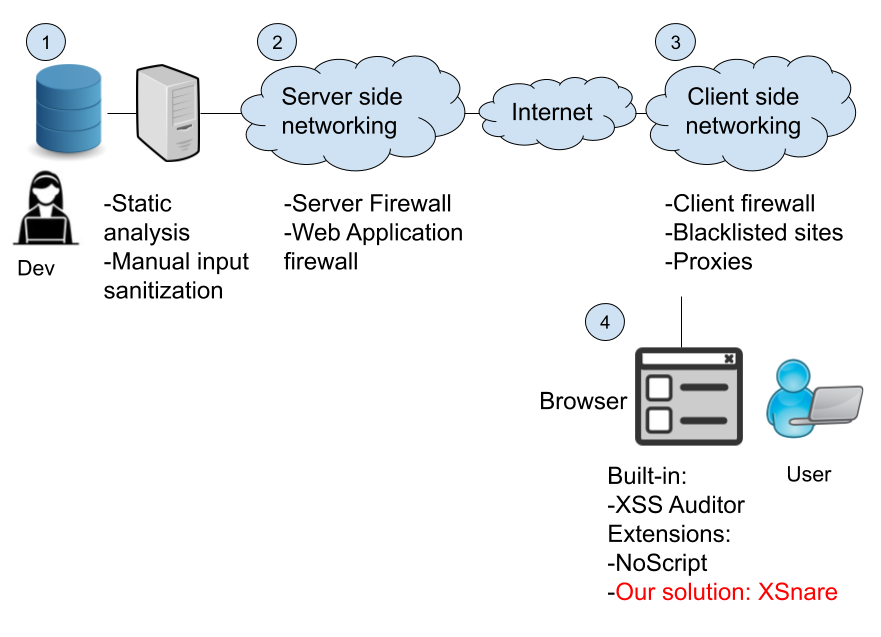
\includegraphics[scale=0.3]{img/web_app_architecture.png}
	\caption{Architecture of typical web applications. Different security solutions apply at distinct layers.}
	\label{fig:web_architecture}
\end{figure}


\subsection{Operation, at a glance}
 Commonly, bug bounty hunters and penetration testers will scour websites to find vulnerabilities and alert developers of issues in these, as well as potential fixes. Developers will then fix the bugs accordingly so that users are not subject to vulnerabilities. Inspired by this workflow, we believe this process can be partly automated using a firewall-based approach, so that users don't have to wait for developers to update their code. Figure~\ref{fig:dom_firewall} illustrates how the firewall can be used to guarantee full client-side protection: A user loads a request, such as www.myblog.com, this request might come back with malicious code in the form of an XSS attack. Before rendering the webpage in the browser, an extension can analyze the potentially malicious document, doing so by loading signatures which a developer (a bug bounty hunter, for example) has uploaded to a database, and completely eliminating the injected code. Finally, the extension returns a clean HTML document, which the browser then renders.
 
 \begin{figure}[h]
 	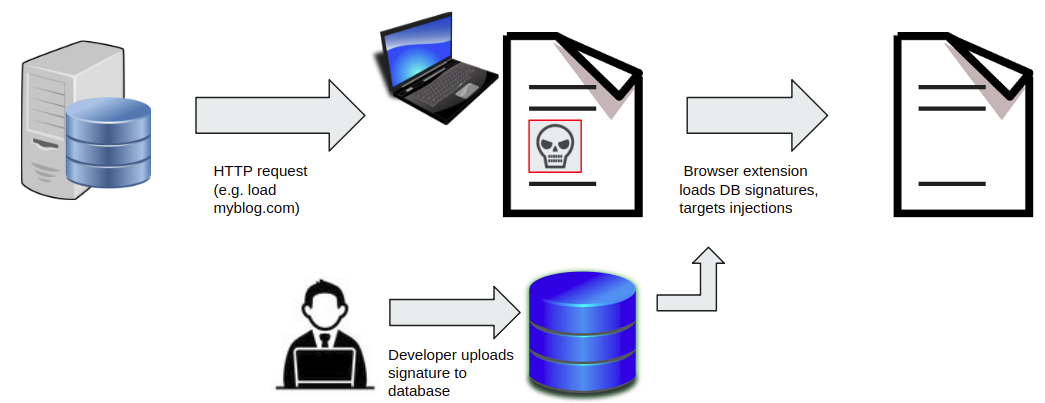
\includegraphics[scale=0.23]{img/dom_firewall.png}
 	\caption{The DOM Firewall approach for protection against XSS.}
 	\label{fig:dom_firewall}
 \end{figure}

\subsection{A simple example}

In order to further illustrate this approach, we present a small example of how DOM context can be used to defend against XSS. This is reproducible in an off-the-box WordPress installation running the Responsive Cookie Consent plugin, v1.7, and Chrome's XSS auditor does not protect against this. Consider a website running PHP on the backend that takes user input and stores it to later display it to another user; in this case, the input element's value attribute is set by the webpage admin using the plugin's UI.

The PHP code defines the static HTML template (in black) in the "admin-page.php" file, as well as the dynamic input (in red):

\begin{lstlisting}
<input id="rcc_settings[border-size]" 
name="rcc-settings[border-size]" 
type="text" value=<@\textcolor{red}{"<?php rcc\_value('border-size'); ?>"}@>/>
<label class="description"
for="rcc_settings[border-size]">
\end{lstlisting}
\
\\
This same HTML will be displayed in the admin's UI. Under normal circumstances, the input element might be used to insert a value of "0" as the dynamic content:
\\
\begin{lstlisting}
<input id="rcc_settings[border-size]" 
 name="rcc-settings[border-size]" 
 type="text" value=<@\textcolor{red}{"0"}@>>
<label class="description"
 for="rcc_settings[border-size]">
\end{lstlisting}
However, if the user is malicious, it could inject a script, as it is not sanitized on the server side. If we have
\begin{lstlisting}
border-size = ""><script>alert('XSS')</script>
\end{lstlisting}
then, the browser will render the following, executing the injected script:
\begin{lstlisting}
<input id="rcc_settings[border-size]" 
name="rcc-settings[border-size]" 
type="text" value=<@\textcolor{red}{""><script>alert('XSS')</script>}@>
<label class="description"
for="rcc_settings[border-size]">
\end{lstlisting}

Note that this HTML is well-formed, so it is hard to detect that a malicious injection has occurred without knowing the developer's intention. However, assuming an analyst has knowledge of how the full HTML should render without any injections, and the possible range of values of the injection, they can single out the point of injection, by separating user input from the server-side template, and get rid of the malicious script entirely. In the example, the injected script in red can be easily distinguished from the rest of the HTML template due to their identifiable attributes. By searching for this specific input element from the top of the document, and this label element from the bottom, the dynamic content can be identified from the static template.

After careful analysis of the code, we noted that while the CVE describing this vulnerability states that the bug was fixed in version 1.8 of this plugin, this was not the case: the developer fixed other similar vulnerabilities but did not handle this specific parameter. However, we can infer the application's intended behaviour from the other patches \cite{rccpatch}. In particular, the developer applied a built-in WordPress function "sanitize\_text\_field", which sanitizes the parameters by checking for common invalid characters like invalid UTF-8. Our system ideally reproduces the developer's intended patch on the client-side. We provide various sanitization techniques to reach this goal.

In the following sections we give a detailed description of each component of our system, the challenges that arise when trying to defend against XSS client-side, and the tools provided by the browser to facilitate our methods. 
 
 \subsection{Firewall Signatures}
	 The firewall signatures are at the core of our defense strategy. These must be precise enough for our system to single out the intended injection, and not an element of the website crucial to the user experience. Since we are only relying on DOM knowledge, these signatures must be related to HTML features, for example, specifying elements and element attributes that are unique to where the exploit might occur. The basis for our signatures relies on two observations: first, an injection has a start and end point, that is, an element can only be injected between a specific HTML node and its immediate sibling in the DOM tree; second, in a well-formed DOM, the dynamic content will not be able to rearrange its location in the document without any JavaScript execution (e.g. removing and adding elements), allowing us to isolate it from the template code. Thus, our basic approach at signature definition is to specify an injection's start and its end, and any sanitization to be done between these two endpoints. Different scenarios might warrant different resolutions, ranging from stopping a webpage's rendering altogether, to performing some basic checks on the string. We discuss how different exploits might affect a signature definition and how our signature language gives an analyst enough expressibility to deal with these in later sections.
	 
	 We believe CVEs to be an ideal source for signatures, and our system assumes these are written by a third-party: as discussed previously, bug bounty hunters and penetration testers will commonly identify issues in application code, inform developers and publish it for the benefit of the community in the form of CVEs. Our system adds an extra component to this workflow, where hackers and security enthusiasts also write the signatures to defend users. Thus, the signature database is maintained by a trusted entity which audits CVEs, and thus, a malicious analyst can not take advantage of this model to throttle the extension's performance. An analyst can write a signature in our language given their knowledge on the exploit, as they will often know both the source and the way it manifests in the HTML, as well as the fix. TODO: feel like this could be expanded but not sure what else to say. Could talk about signature sharing for power-users to get back to the user-centred argument, although we haven't really gotten this far into deployment talk yet.
 
 \subsection{Firewall Signature Language}
 Our signature language needs to be such that it has enough power of expression for the signature writer to be precise. Due to the nature of our signature definitions, a regex language suffices to express precise sections of the HTML. Furthermore, a regex language allows us to identify malformed HTML before it renders on the browser. The following is the signature that defends against the motivating example of Section 2.1:
 \lstset{basicstyle=\small}
\begin{lstlisting}
url: 'wp-admin/options-general.php?page=rcc-settings',
software: 'WordPress',
softwareDetails: 'responsive-cookie-consent',
version: '1.5',
type: 'string',
typeDet: 'single',
sanitizer: 'regex',
config: '/^[0-9](\.[0-9]+)?$/',
endPoints: 
['<input id="rcc_settings[border-size]" 
name="rcc_settings[border-size]" type="text" value="',
'<label class="description" 
for="rcc_settings[border-size]">']
\end{lstlisting}
 
 Along with the previously mentioned endpoints, the signature also defines the urls, if necessary, in which the exploit occurs, what kind of webpage it is (WordPress in this case), and any additional details of the software. In this case, since it's a WordPress site, the details include the description of the vulnerable plugin. The typeDet value specifies whether this signature includes a "single" pair of endPoints, or "multiple". This is useful for when one signature developer has identified several vulnerable points in the same document, and the writing can be streamlined into one signature. Having multiple injection points in one document complicates the detection mechanism: for example, if one document has two different injection points, a knowledgeable attacker might leverage this information to try to trick the extension into identifying the wrong spots. We further discuss measures to protect against these attacks in the implementation section.
 
 \subsection{Firefox Extension}
Our extension's main purpose is to detect exploits in the HTML by using signature definitions and maintain a local database of signatures that is periodically updated from the main server.
The extension model provided by several browsers allows us to interpose on any functionality of a website in a privileged execution environment, unavailable to any third-party. In particular, Firefox provides the filterResponseData method through the webRequest API \cite{webRequest} . This allows the extension's background page to analyse and modify incoming network traffic. The extension therefore translates signature definitions into the logic needed to rewrite incoming HTML on a per-URL basis, according to the top-down, bottom-up scan described earlier. 

A network filter is particularly useful in the case of client-side XSS (e.g. DOM Based XSS), and to detect malformed HTML or detect XSS before it can rearrange itself in the HTML. For example, a <tr> element may only have direct children <th> or <td>. In our experiments, we found that an injection occurring as a direct child of the <tr> might cause the injected element to be rendered before the <tr> in the DOM. This defies one of our key observations with regards to injection placements. Therefore, we can't wait until the website is rendered client-side to start interposing on code execution.

This approach guarantees safety even in the face of a knowledgeable attacker: if they know what the signatures look like, they can't take advantage of this knowledge because the extension can't be tricked into looking for the element in the wrong spot, as the injection can only happen after a signature's start and before its end. Since the injection can't be infinitely long, it can be easily distinguished from the HTML template.


\iffalse
While we haven't seen any examples that warrant this functionality, it is possible for an exploit to only manifest itself through client-side dynamic behaviour, i.e. after an user clicks on the page. The network filter might not be able to defend against this, but the extension's content script can safely interpose on it through the user of event listeners and in particular Firefox's \textbf{beforescriptexecute} event, which occurs before a script element executes. Signatures can also be defined for these scenarios, to be ran in the content script. However, we believe this to be less ideal due to the added performance costs, as the extension now has to install the content script's code on all browser tabs.
\fi



